\chapter{Samplers: Framework Android}




\section{Jerarquía de Clases}
Nuestras clases, las que permiten que se cree una app

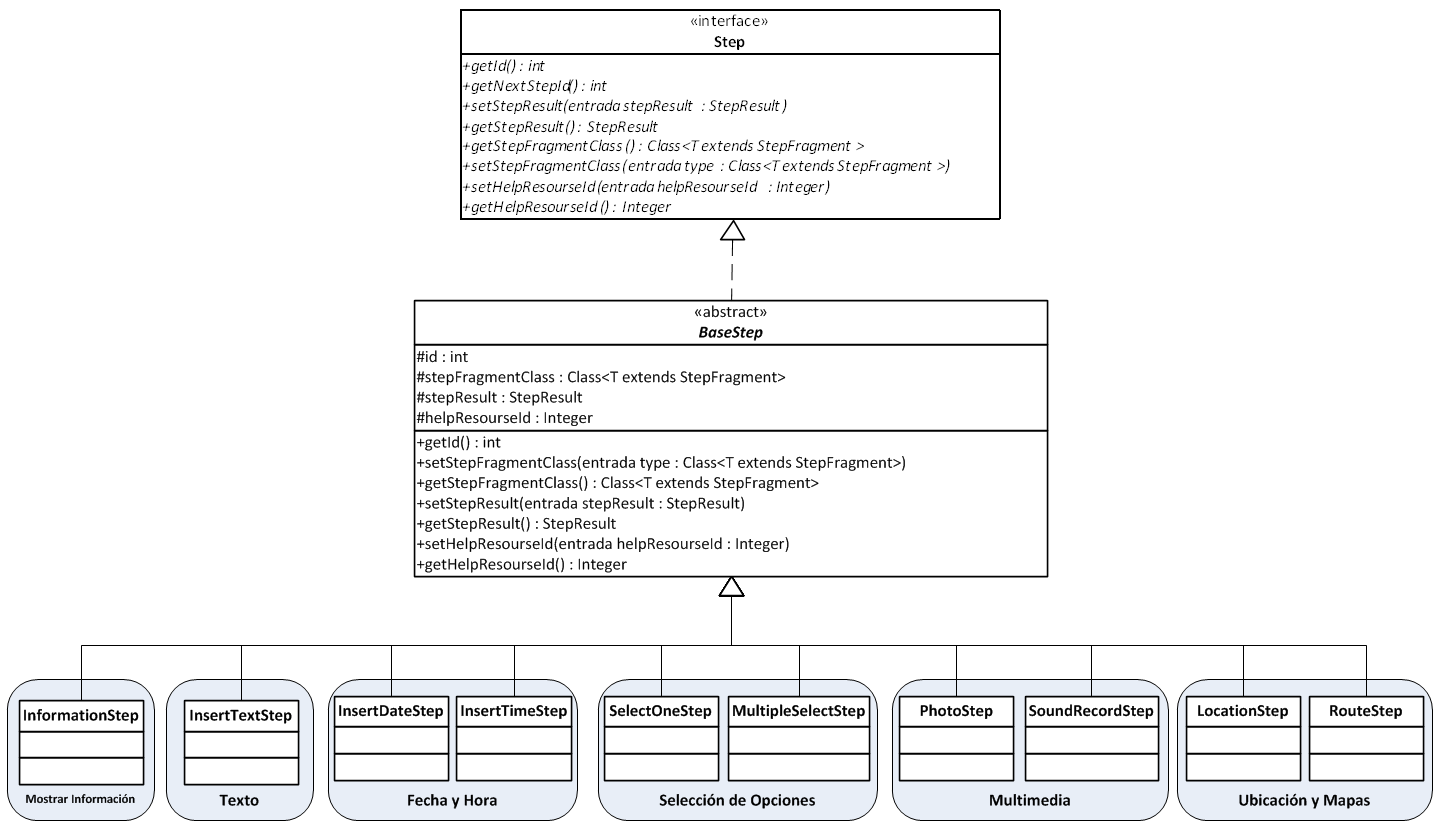
\includegraphics[scale=0.4]{05-implementacion/Steps.png} 


\subsection{Workflow: Control de Ejecución}

\subsubsection{Step, el Paso}

\subsubsection{StepResult, El Resultado de la Ejecución del Paso}

\subsubsection{Muestra, Conjunto de Resultados}

\subsection{Envío de Muestras a Servidor Web}
Acá explicamos un poco la estrategia que utilizamos para el envío de muestras y las librerías externas que nos ayudaron.

\section{Instalación y uso del framework}
Instalación. 
Requerimientos mínimos:
\begin{itemize}
\item Android Studio (Java): Si bien esta pensado para y probado en Android Studio, podria funcionar bien en otro entorno que use Java y deje importar archivos Android Archive (.aar).
\item Android SDK API17: Android 4.2 (Jelly Bean) o superior.
\end{itemize}

Instalación:
\begin{enumerate}
	\item Crear en Android Studio un nuevo proyecto vacío (sin ninguna Activity).
		\begin{itemize}
		\item Seleccionar API17 o superior como versión mínima de Android SDK
		\end{itemize}
	\item Importar la librería del framework en el proyecto creado
		\begin{itemize}
		\item Descargar la última versión de samplersFramework.aar desde https://github.com/			cientopolis/samplers/releases/
		\item Importar la librería al proyecto: File -> New -> New Module -> Import .JAR/.AAR Package
		\end{itemize}
	\item Agregar el repositorio de Google
		\begin{itemize}
			\item En el archivo build.gradle del proyecto agregar: 
			\begin{lstlisting}[language=XML, frame=single]
allprojects {
    repositories {
        jcenter()
        google()
    }
}
			\end{lstlisting}	
		\end{itemize}
	\item Agregar las dependencias necesarias:
		\begin{itemize}
			\item En el archivo build.gradle de la aplicación agregar: 
			\begin{lstlisting}[language=XML, frame=tlb]
dependencies {
  // here the standards dependencies created by Android Studio
  // ...

  // if not added automatically, add this dependency 
  // you should use the latest version e.j. 25.+
  compile 'com.android.support:design:24.2.1' 
  compile 'com.android.support.constraint:constraint-layout:1.0.2'

  // if you will use maps and location services, add this dependencies (you should use the latest version)
  compile ('com.google.android.gms:play-services-location:12.0.1')
  compile ('com.google.android.gms:play-services-maps:12.0.1')
  
  // if you will use authentication with Google, add this dependencies (you should use the latest version)
  compile ('com.google.android.gms:play-services-auth:12.0.1')

  // the framework dependency
  compile project(":samplersFramework")
}
			\end{lstlisting}	
		\end{itemize}	

	\item Instanciar:
		\begin{itemize}
		\item La instanciación puede ser manual o usando el generador de clases en Gradle como se explica en la siguiente sección.
		\end{itemize}
\end{enumerate}	

\subsection{Instanciación}
Una vez instalado el framework...
La instanciación puede ser manual o usando el generador de clases de Gradle.

\subsubsection{Instanciación manual}
Básicamente se tiene que crear un objeto Workflow, agregarle los objetos Steps, y llamar a la activity TakeSampleActivity pasándole el workflow como parámetro.
También es necesario establecer la configuración general en el método onCreate de la activity principal (main activity).
Se puede usar una activity principal propia o se puede heredar de SamplersMainActivity. En ambos casos se debe hacer lo siguiente:
\begin{itemize}
	\item Establecer la configuración general en el método onCreate de la activity principal:
		\begin{lstlisting}[language=Java, frame=tlb]
NetworkConfiguration.setURL("http://192.168.1.10/samplers/upload.php");
NetworkConfiguration.setPARAM_NAME_SAMPLE("sample");
// Optional if you will use authentication
NetworkConfiguration.setPARAM_NAME_USER_ID("user_id");
NetworkConfiguration.setPARAM_NAME_AUTHENTICATION_TYPE("authentication_type");

// Optional if you will use authentication, set the configuration
AuthenticationManager.setAuthenticationEnabled(true);
AuthenticationManager.setAuthenticationOptional(true);
		\end{lstlisting}

	\item Crear un Workflow. Si se está heredando de SamplersMainActivity se debe hacer sobreescribiendo el método onCreate.
		\begin{lstlisting}[language=Java, frame=tlb]
@Override
protected Workflow getWorkflow() {
	Workflow workflow = new Workflow();
    	
	Step step = new InformationStep(2,"Por favor tome una foto de su gato", null);
	workflow.add(step);
    	
	step = new PhotoStep(1,"Bienvenido a la app de prueba", 2);
	workflow.add(step);
    	
	return workflow;
    	
}		
		\end{lstlisting}
Nota: en el ejemplo anterior se muestra un Workflow que tiene dos Steps. El primero muestra un mensaje de bienvenida y el segundo pide para tomar una foto. Para ver los distintos Steps que se pueden usar vea la sección de Steps.

	\item Iniciar la activity TakeSampleActivity. Si se está heredando de SamplersMainActivity esto se hace solo en el método onClick del botón "tomar muestra". De lo contrario, deberá iniciarla de la siguiente forma, en el método onClick de un botón por ejemplo:
		\begin{lstlisting}[language=Java, frame=tlb]
@Override
public void takeSampleClick(View view) {
	Workflow workflow = getWorkflow();

	Intent intent = new Intent(this, TakeSampleActivity.class);        
	intent.putExtra(TakeSampleActivity.EXTRA_WORKFLOW, workflow);
	startActivity(intent);
    	
}		
		\end{lstlisting}




\end{itemize}


\subsubsection{Instanciación usando el  generador de clases de Gradle}

Básicamente, el generador de clases de Gradle se encarga de hacer una instanciación manual a partir de un archivo de configuración (JSON). Está pensado para desarrolladores que no tienen muchos conocimientos en Android, o para servir de interfaz entre una aplicación que genere apps a través de Samplers (esto hay que escribirlo mejor).

Los pasos para usar el generador de clases de Gradle son:
\begin{enumerate}
	\item Crear un archivo JSON con el nombre SamplersConfig.json
		\begin{itemize}
			\item El formato y las opciones están explicadas en la siguiente sección.
			\item Para validar sintaxis se puede usar el validador online: jsonformatter.curiousconcept.com (Ver si se puede poner esto o hay que tener permisos?)
			\item Al final de la sección se provee un archivo de ejemplo
		\end{itemize}
		
	\item Copiar el archivo creado en el item anterior al directorio raíz del proyecto Android
	
	\item Descargar la última versión de los archivos \textbf{samplers.gradle} y \textbf{samplersclassgenerator.jar} del repositorio de Samplers (https://github.com/cientopolis/samplers/releases/) y copiarlos también al directorio raíz del proyecto Android
	
	\item Enlazar el archivo samplers.gradle en el archivo build.gradle de la aplicación
		\begin{itemize}
			\item Android Studio crea por defecto dos archivos build.gradle, uno a nivel de aplicación y otro a nivel de proyecto. Debe usarse el de aplicación
			\item Al final del archivo build.gradle de aplicación agregar:
\begin{lstlisting}[language=XML, frame=tlb]
apply from: '../samplers.gradle'
\end{lstlisting}
			\item Al guardar los cambios, Android Studio sugerirá hacer una sincronización del proyecto, hacerla. Esto generará en la aplicación una activity llamada MyMainSamplersActivity en base a las opciones configuradas en el archivo SamplersConfig.json.
			\item Si se necesita volver a generar esta activity (si se quieren modificar algunas opciones por ejemplo ) se puede eliminar la misma, hacer las modificaciones en el archivo SamplersConfig.json y volver a generar el proyecto (en el menu Build -> Make Project)
		\end{itemize}
		
	\item Eliminar o (customizar) el archivo \textbf{style.xml} que está en \textbf{res/values} en la aplicación
	
	\item Ejecutar la aplicación y listo.

\end{enumerate}


\subsection{Secciones del Archivo}

El archivo SamplersConfig.json es un archivo JSON con 3 objetos:
\begin{itemize}
	\item El objeto \textbf{project}
	\item El objeto \textbf{application}
	\item El objeto \textbf{workflow}
\end{itemize}


\subsubsection{Configuración de los Servicios de Google}

\section{Generador de Clases}